\begin{flushright} {\tiny {\color{gray} axisymmetric\_eqs.tex}} \end{flushright}
%~~~~~~~~~~~~~~~~~~~~~~~~~~~~~~~~~~~~~~~~~~~~~~~~~~~~~~~~~~~~~~~~~~~~~~~~~~~~~~~~~~~~~~~~~~~~~~~~~~

In what follows we are concerned with incompressible flow.
In some cases the assumption can be made that the object we wish to sudy has an 
axisymmetric geometry, for example a plume:

\begin{center}
a)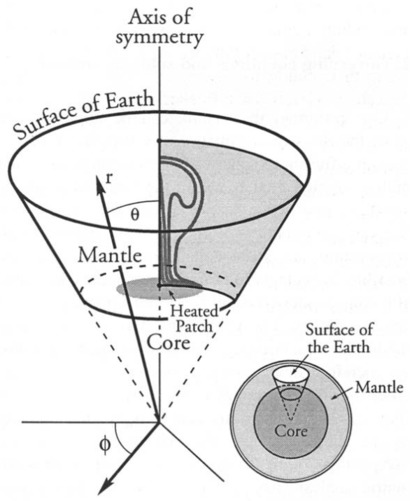
\includegraphics[width=5cm]{images/axisymmetry/keki97}
b)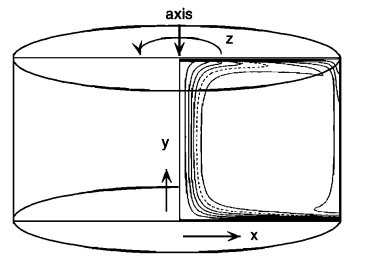
\includegraphics[width=5cm]{images/axisymmetry/lesy96a}
c)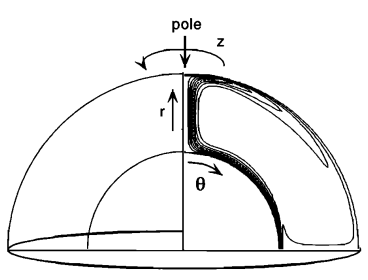
\includegraphics[width=5cm]{images/axisymmetry/lesy96b}\\
{\captionfont a)Taken from Kellogg \& King (1997) \cite{keki97}.
b,c) Taken from Leitch \etal (1996) \cite{lesy96}.}
\end{center}

Looking at the figure above we see that there are in fact two cases: axisymmetry in 
cylindrical coordinates (b) and axisymmetry in spherical coordinates (c).

As mentioned in Kellogg \& King (1997) \cite{keki97}: "By imposing axisymmetry,
we restrict the problem to two degrees of freedom, reducing the computational
effort significantly over 3D calculations."
However, Redmond \& King (2004) \cite{reki04} also mention:
"An important caveat of axisymmetric calculations is that there are no variations 
in the $\phi$ direction (i.e., there are no $\phi$ derivatives in
the governing equations). Thus, as we get further from
the pole, the results become increasingly less physical.
Downwelling drips off the pole are actually downwelling
doughnuts that follow the entire small circle. In a fully
3D calculation, this doughnut feature would in reality be a drip."


See Section~\ref{ss:cyl_axi} for the FE formulation of these equations.

%---------------------------------------
\subsubsection{In cylindrical coordinates}

The velocity vector is $\vec{\upnu}=(\upnu_r,\upnu_\theta,\upnu_z)$. 
Due to the symmetry we have $\upnu_\theta=0$, $\partial_\theta \rightarrow 0$ 
and the Stokes equations 
then become \footnote{\url{https://en.wikipedia.org/wiki/Navier-Stokes_equations}}

\begin{eqnarray}
-\frac{\partial p}{\partial r} + \eta
\left(
\frac1r \frac{\partial}{\partial r} ( r  \frac{\partial \upnu_r}{\partial r}   ) 
+  \frac{\partial^2 \upnu_r}{\partial z^2} - \frac{\upnu_r}{r^2}
\right) +\rho g_r&=& 0 
\\
-\frac{\partial p}{\partial z} + \eta
\left(
\frac1r \frac{\partial}{\partial r} ( r  \frac{\partial \upnu_z}{\partial r}   ) 
+  \frac{\partial^2 \upnu_z}{\partial z^2} 
\right) +\rho g_z&=& 0 \\
\frac1r \frac{\partial}{\partial r} (r \upnu_r) + \frac{\partial \upnu_z}{\partial z} &=& 0
\end{eqnarray}


The strain rate tensor in cylindrical coordinates is given by 

\begin{eqnarray}
\dot\varepsilon_{rr} 
&=& \frac{\partial \upnu_r}{\partial r} 
\\
\dot\varepsilon_{\theta\theta} 
&=& \frac{\upnu_r}{r} + \frac{1}{r} \frac{\partial \upnu_\theta}{\partial \theta}  
\\
\dot\varepsilon_{\theta r} = \dot\varepsilon_{r\theta} 
&=& \frac{1}{2} \left(   \frac{\partial \upnu_\theta}{\partial r} - \frac{\upnu_\theta}{r} 
+\frac{1}{r} \frac{\partial \upnu_r}{\partial \theta}  \right)
\\
\dot\varepsilon_{zz} 
&=& \frac{\partial \upnu_z}{\partial z} 
\\
\dot{\varepsilon}_{rz} = \dot{\varepsilon}_{zr} 
&=& \frac{1}{2}\left( \frac{\partial \upnu_r}{\partial z} + \frac{\partial \upnu_z}{\partial r}  \right) 
\\
\dot{\varepsilon}_{\theta z} = \dot{\varepsilon}_{z \theta} &=& \frac{1}{2}\left( 
\frac{1}{r} \frac{\partial \upnu_z}{\partial \theta} + \frac{\partial \upnu_\theta}{\partial z}  \right) 
\end{eqnarray}

In the axisymmetric case, we have $\upnu_\theta=0$ and $\partial_\theta \rightarrow 0$ so that 
\begin{eqnarray}
\dot\varepsilon_{rr} &=& \frac{\partial \upnu_r}{\partial r}  \\
\dot\varepsilon_{\theta\theta} &=& \frac{\upnu_r}{r} \\
\dot\varepsilon_{r\theta} = \dot\varepsilon_{\theta r} &=& 0\\
\dot\varepsilon_{zz} &=& \frac{\partial \upnu_z}{\partial z} \\
\dot{\varepsilon}_{rz} = \dot{\varepsilon}_{zr} 
&=& \frac{1}{2}\left( \frac{\partial \upnu_r}{\partial z} + \frac{\partial \upnu_z}{\partial r}  \right) \\
\dot{\varepsilon}_{\theta z} = \dot{\varepsilon}_{z \theta} &=& 0
\end{eqnarray}
or, 
\[
\dot{\bm\varepsilon}
=
\left(
\begin{array}{ccc}
\dot\varepsilon_{rr} & 0 & \dot{\varepsilon}_{rz} \\
0 & \dot{\varepsilon}_{\theta\theta}  & 0 \\
\dot{\varepsilon}_{zr} & 0 & \dot\varepsilon_{zz}
\end{array}
\right)
\]

See for example Kiefer \& Hager (1992) \cite{kiha92}.




%---------------------------------------
\subsubsection{In spherical coordinates}




Assuming the flow velocity does not depend on $\phi$ ($\partial_\phi =0$) and therefore also that $\upnu_\phi=0$
\[
0=-\frac{\partial p}{\partial r} + f_r + \eta \left(\Delta v_r - \frac{2v_r}{r^2} -\frac{2}{r^2} \frac{\partial v_\theta}{\partial \theta} - \frac{2 v_\theta \cot \theta }{r^2} \right)
\]
\[
0 = -\frac{1}{r} \frac{\partial p}{\partial \theta} + \eta \left(\Delta v_\theta + \frac{2}{r^2} \frac{\partial v_r}{\partial \theta}  - \frac{v_\theta}{r^2 \sin^2 \theta} \right)
\]
with
\[
\Delta = \frac{1}{r^2} \frac{\partial }{\partial r}\left( r^2 \frac{\partial }{\partial r}\right)
+\frac{1}{r^2 \sin\theta} \frac{\partial }{\partial \theta}
\left(
\sin\theta \frac{\partial }{\partial\theta}
\right)
\]


\[
\Delta = \frac{1}{r^2} \frac{\partial }{\partial r}\left( r^2 \frac{\partial }{\partial r}\right)
+\frac{1}{r^2 \sin\theta} \frac{\partial }{\partial \theta}
\left(
\sin\theta \frac{\partial }{\partial\theta}
\right)
+ \frac{1}{r^2 \sin^2\theta} \frac{\partial^2 }{\partial\phi^2}
\]

THESE EQUATIONS SHOULD BE CHECKED and RE-CHECKED !!



From \cite{zebi93}:
\begin{equation}
\frac{1}{r^2} \frac{\partial}{\partial r} (r^2 \upnu_r) + 
\frac{1}{r \sin \theta} \frac{\partial}{\partial \theta} (\upnu_\theta \sin \theta)+
\frac{1}{r \sin \theta} \frac{\partial \upnu_\phi}{\partial \phi} = 0
\end{equation}
Pb with 1/r2 ??

\begin{eqnarray}
0 &=& -\frac{\partial p}{\partial r} + (1-\zeta) Ra \; r \; T + 
\frac{1}{r^2}\frac{\partial}{\partial r} \left( 2 \eta r^2 \frac{\partial \upnu_r}{\partial r} \right)
+ \frac{1}{r^2 \sin\theta} \frac{\partial}{\partial\theta} 
\left( \eta \sin\theta \frac{\partial \upnu_r}{\partial\theta} \right)
+\frac{\partial}{\partial \theta} \left(\eta \frac{\partial}{\partial r} \frac{\upnu_\theta}{r} \right)
\end{eqnarray}
where $\zeta=R_i/R_o$


The dimensional form of the energy equation in a spherical axisymmetric geometry is given by
(assuming the conductivity $k$ to be constant):
\[
\rho C_p \left( \frac{\partial T}{\partial t}  + 
\upnu_r \frac{\partial T}{\partial r} + \frac{\upnu_\theta}{r} \frac{\partial T}{\partial \theta}
\right)
=
k \frac{1}{r^2} \frac{\partial}{\partial r} \left( r^2 \frac{\partial T}{\partial r} \right)
+
k \frac{1}{r^2 \sin\theta} 
\frac{\partial}{\partial \theta} \left( \sin\theta \frac{\partial T}{\partial \theta}  \right) 
...
\]

THESE EQUATIONS SHOULD BE CHECKED and RE-CHECKED !!



